\subsubsection{Latency and Buffer}

To project analog vibrations to the speakers,  the audio hardware needs to convert this digital signal to
continuous analog voltage using Digital-to-Analog Conversion (DAC). And vice-versa for the microphones using
Analog-to-Digital (ADC) converter. \Cref{fig:latency_signal_flow} presents a simplified signal flow diagram illustrating 
the sources of latency in a digital audio system consisting of ADC and DAC conversion down to buffering and 
processing \cite{burg2014latency}.

\begin{figure}[ht]
  \centering
  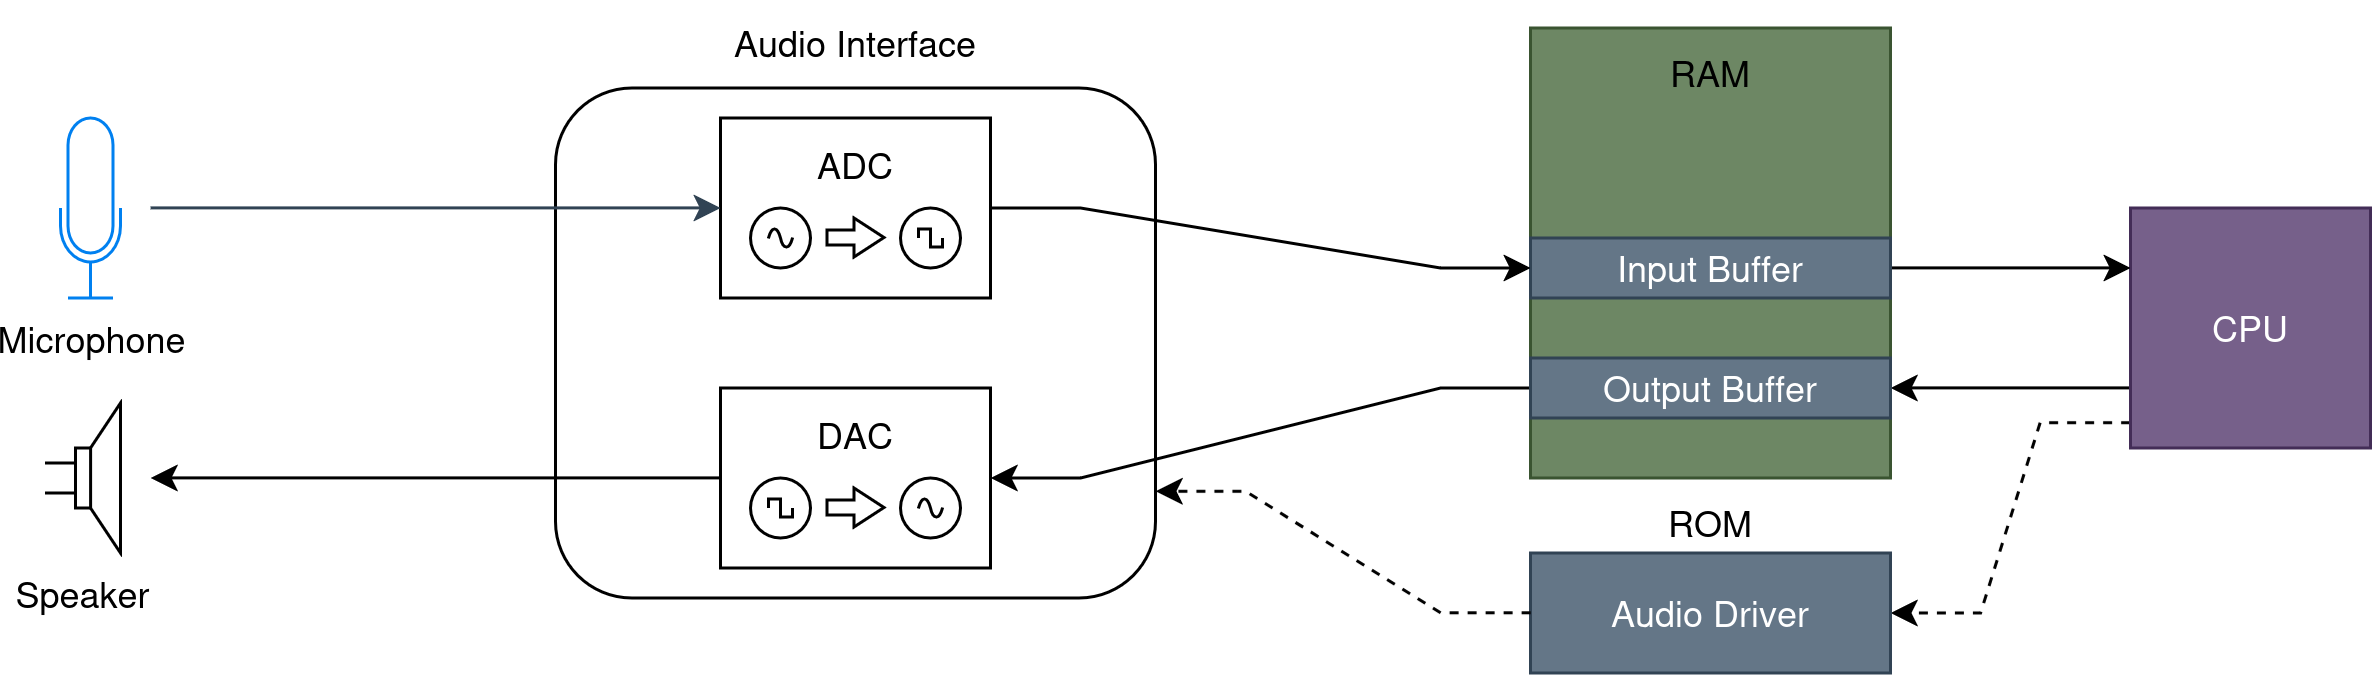
\includegraphics[width=\linewidth]{discussion/audio_basics/figures/SignalFlowDiagramDAC.drawio.png}
  \caption{Signal flow during the latency period \cite{burg2014latency}}
  \label{fig:latency_signal_flow}
\end{figure}

This introduces some latency at regular intervals which causes this delay. However, there are other contributing factors which leads
to such delays (\Cref{prompt:latency_factors}) \cite{openai_chatgpt}:

\begin{itemize}
    \item \textbf{Driver / OS scheduling}: Transfer of data between the audio driver and the application
    \item \textbf{DAW Software Processing}: Time taken by the callback or audio engine to synthesize audio and apply DSP 
    (EQ, convolution, compressors, etc.). It depends on the complexity, which is discussed in the later subsections.
    \item \textbf{I/O Buffer Size}: The larger the number of samples queued, the more time it takes to process those signals 
\end{itemize}

The buffer size is one of the largest contributors to latency, i.e. the time taken to process all the samples after being 
queued to a block of memory. Using solely the buffer size, the latency can be modelled using the equation \cite{burg2014latency}:

\begin{equation}\label{eq:buffer_latency}
    t_{\text{buffer}} = \frac{ N_{\text{buffer}} }{f_s}
\end{equation}

Where $N_{\text{buffer}}$ is the buffer size, and $f_s$ is the sampling frequency. For example, for a buffer size of 256 
samples and a sample rate of 48 kHz, the buffer duration would be,

$$
\frac{256}{48000} \approx \SI{5.33}{\milli \second}
$$